\section{Results} \label{sec:Results}

\lipsum[17]

See \fig{plot1SC}, \fig{plot1}, \fig{plot2}, \fig{plot3} and \fig{plot1N}.

\begin{SCfigure}[0.75][h!tbc]
        \centering
                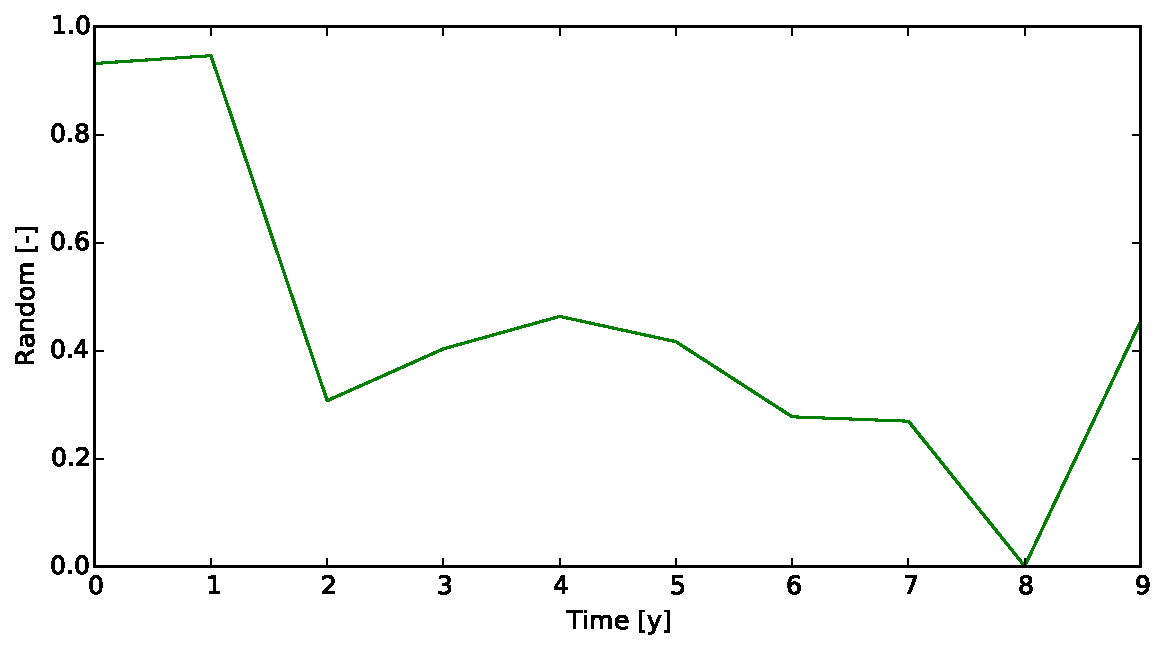
\includegraphics[width=0.48\textwidth]{plot1}
				\caption{Side Cap figure \capunit{\celsius}.
				\label{fig:plot1SC}}
\end{SCfigure}

\lipsum[18]




\singlefig{plot1}{singlefig: Caption}

\doublefig{plot2}{doublefig: Caption 1}{plot3}{doublefig: Caption 2}

\lipsum[18]



\begin{figure}[h!tbc]
        \centering
        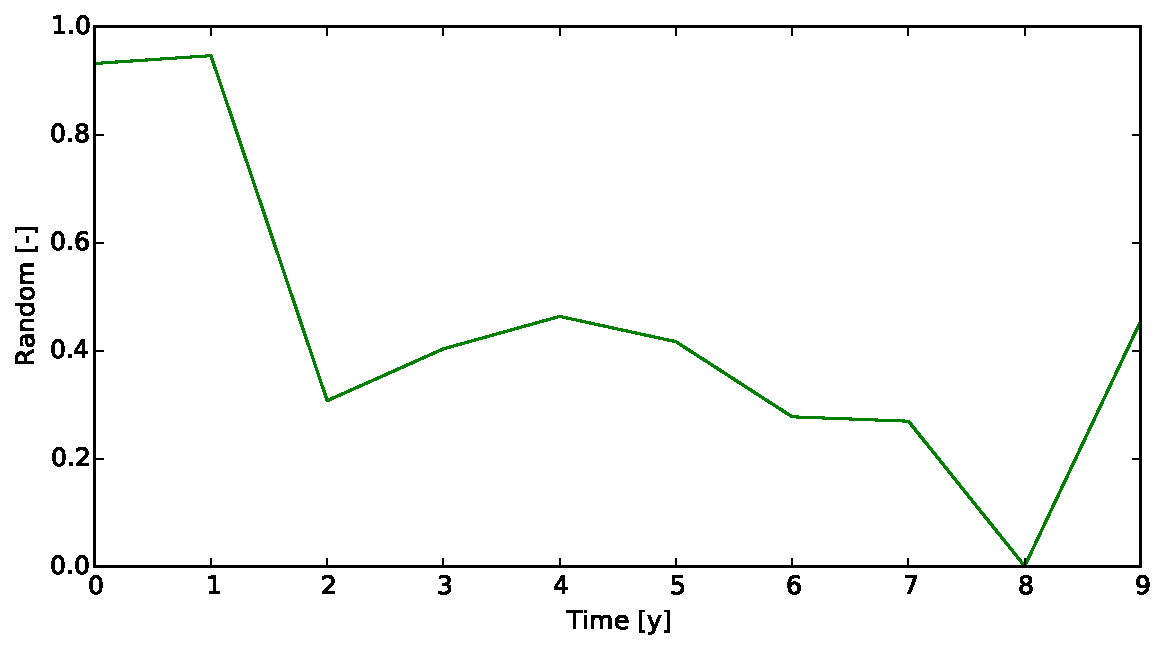
\includegraphics[width=\textwidth]{plot1}   
	\caption{Normal figure. \label{fig:plot1N}}
\end{figure}


\lipsum[19]

\begin{figure}[h!tbc]
\begin{tikzpicture}
\begin{axis}[scale only axis, width=0.1pt, height=0.1pt, ymin=0, ymax=3, xmin=0, xmax=5, ticks=none, ytick = \empty, legend style = {font=\sansmath\sffamily\small}, area legend, legend pos=south west, axis lines = none,legend to name = leg,legend columns = -1]

% LEGEND
	\addlegendimage{black,fill= red}
	\addlegendimage{black,fill= white}
	\addlegendimage{black,fill= blue}
	\addplot coordinates{(0,0)};
		\legend{{$\Delta$LH $> 0$\hspace*{2pt}},{$\Delta$LH $\approx 0$\hspace*{2pt}}, $\Delta$LH $< 0$}
	\end{axis}


	\node[inner sep = 0pt] (fig) {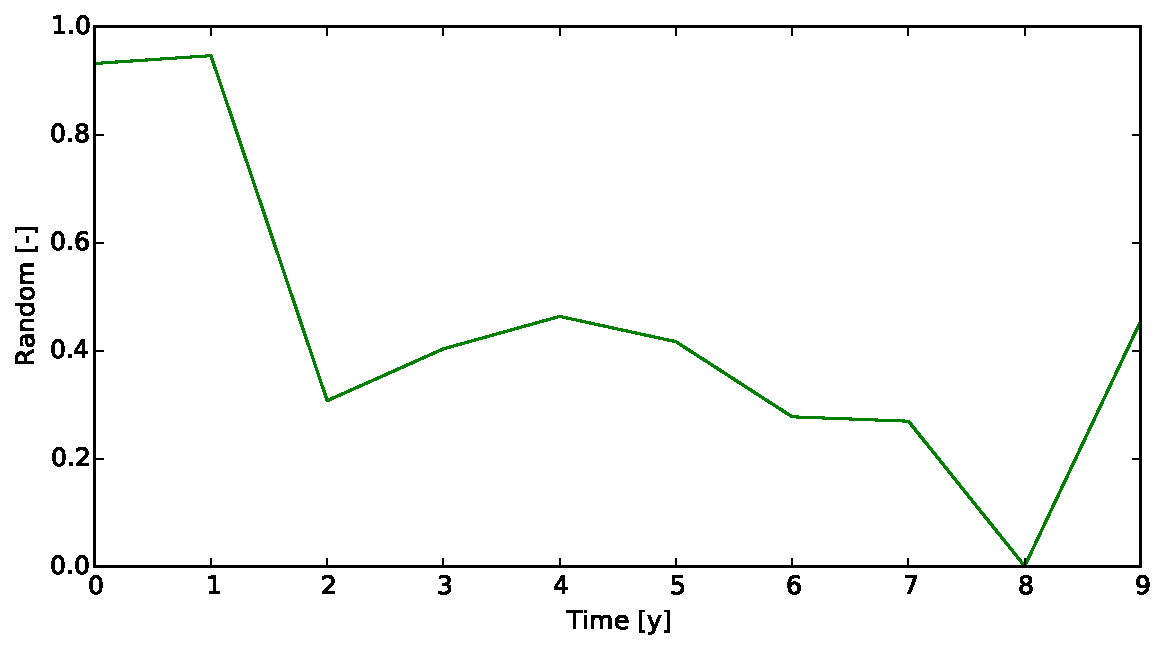
\includegraphics[angle=0,width=\textwidth]{plot1}};

\path[draw,semithick,white] (fig.south west) ++(1.31,2.11) rectangle +(0.3cm,0.3cm);

\node[below] at (fig.south) {\pgfplotslegendfromname{leg}};

% INSET

\node[anchor=south west,xshift=2.5cm,yshift=1.5cm] (ct) at (fig.south west) {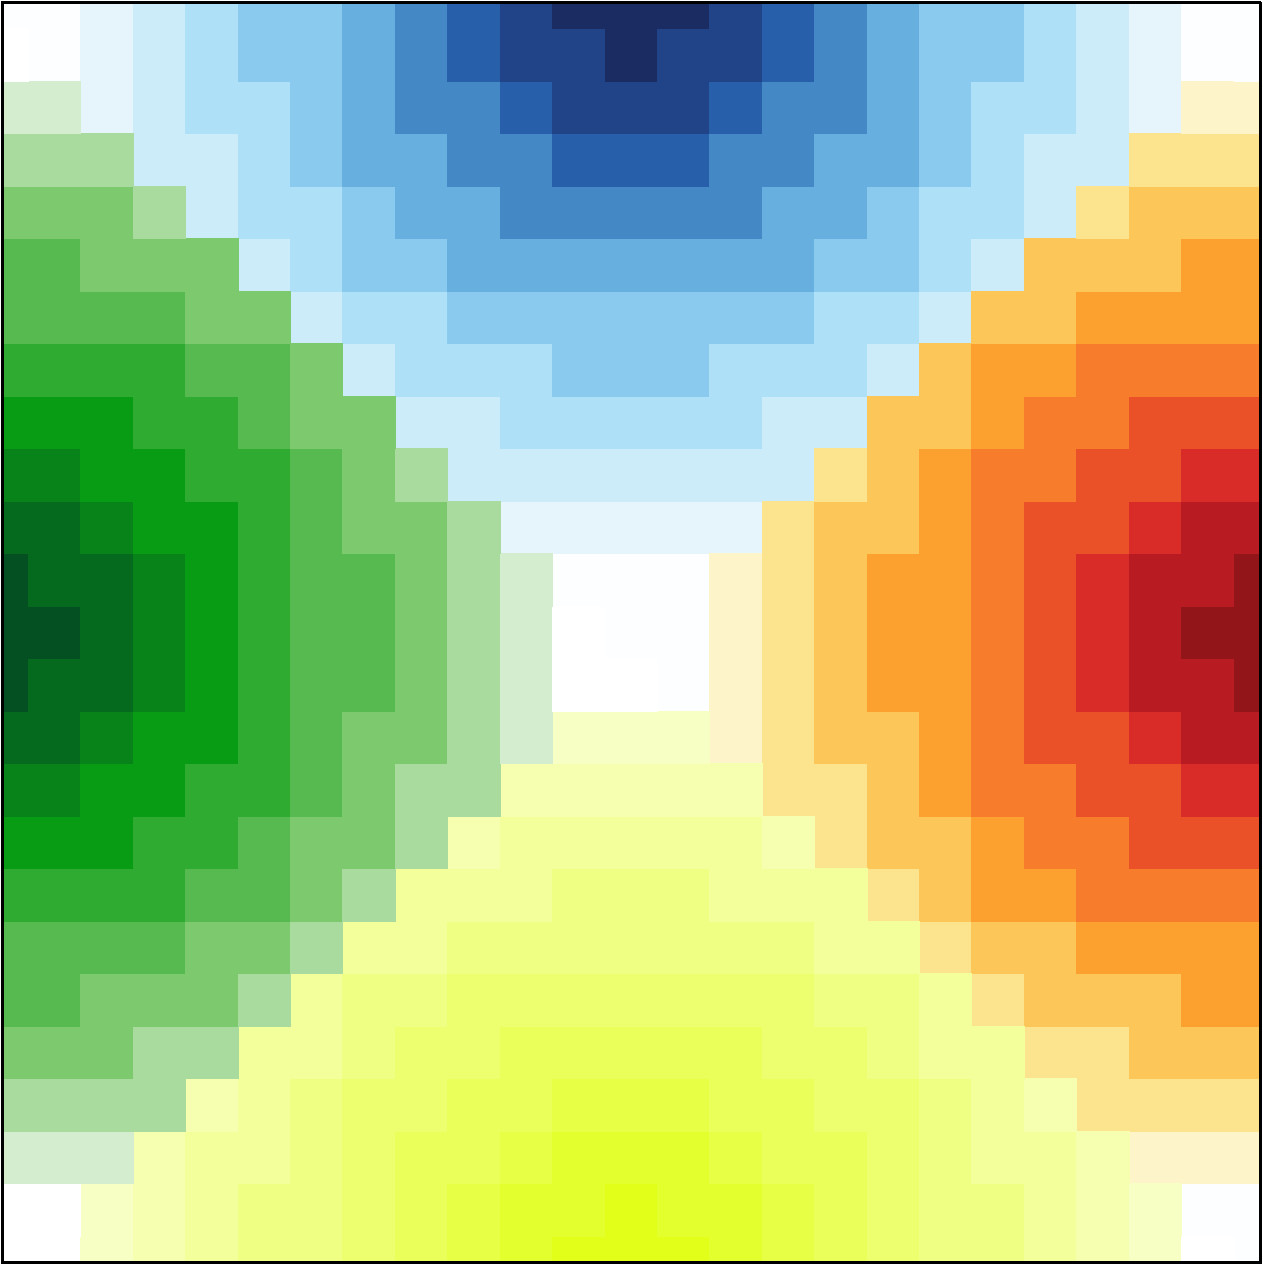
\includegraphics[width=0.1\textwidth]{colortable}};
\begin{scope}[font = \scriptsize\sansmath\sffamily, inner sep = 2pt]
	\begin{scope}[left]
		\node at (ct.north west) {$1$};
		\node (rhoSW) at (ct.west) {$0$};
		\node at (ct.south west) {$-1$};
	\end{scope}
	\node[rotate=90,above] at (rhoSW.west) {$\rho_{LH, SW}$};

	\begin{scope}[above]
		\node at (ct.north west) {$-1$};
		\node (rhoP) at (ct.north) {$0$};
		\node at (ct.north east) {$1$};
	\end{scope}
	\node[above] at (rhoP.north) {$\rho_{\text{LH,P}}$};
\end{scope}
\end{tikzpicture}

\captionof{figure}{Hand-made legend with pgfplots and labeled inset with tikz.}				
 
\end{figure}



\lipsum[20]


\subsection{Water Balance} \label{sec:wBal}

\lipsum[21]

\begin{figure}[h!tbc]
\begin{tikzpicture}
\node (CTRL)    {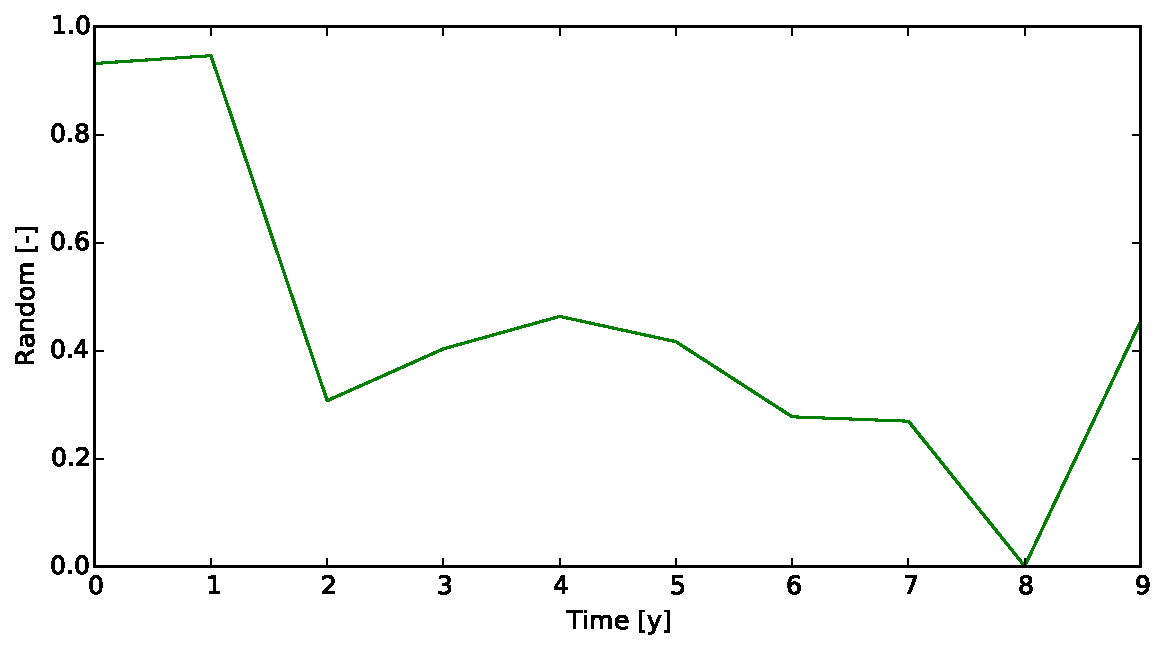
\includegraphics[width=0.310\textwidth]{plot1}};
\node[anchor=south west] (MIN) at (CTRL.south east) {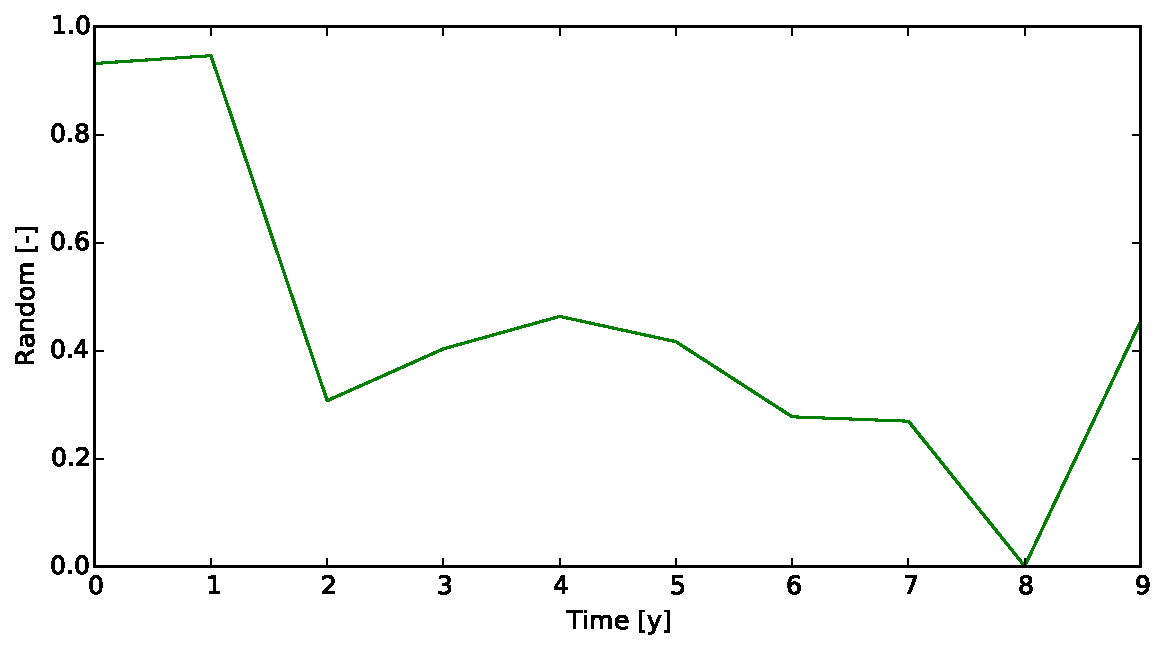
\includegraphics[width=0.310\textwidth]{plot1}};
\node[anchor=south west] (MAX) at (MIN.south east)   {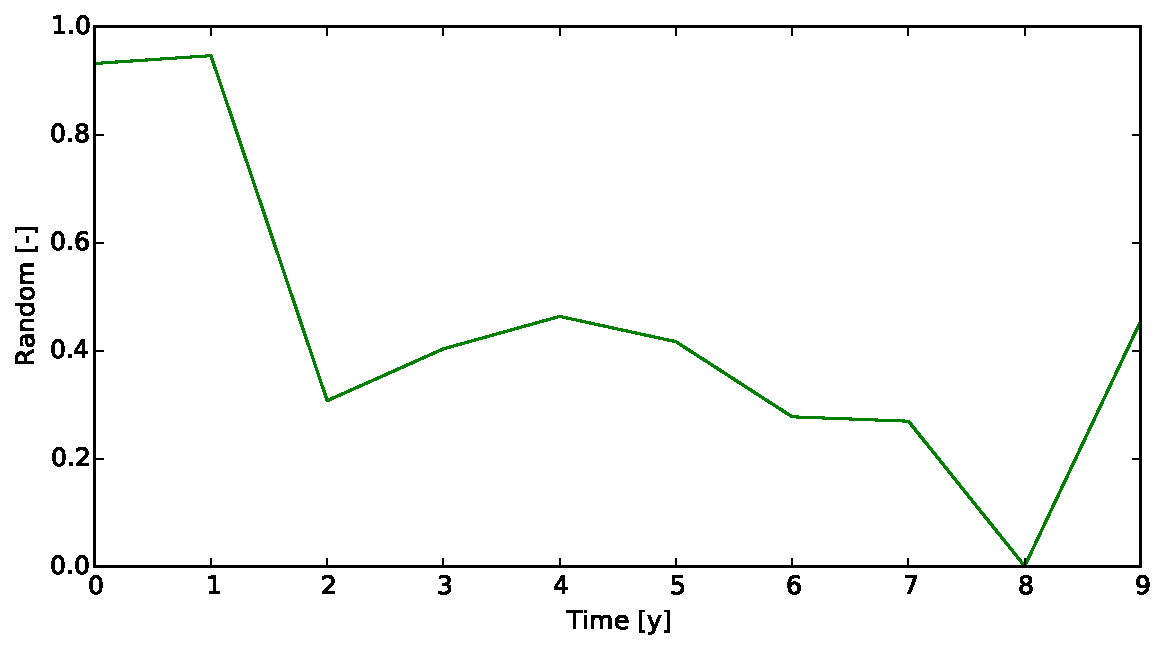
\includegraphics[width=0.310\textwidth]{plot1}};
\node[anchor=north,font=\sansmath\sffamily\small] at (CTRL.north west) {(a)};
\node[anchor=north east,font=\sansmath\sffamily\small] at (MIN.north west) {(b)};
\node[anchor=north west,font=\sansmath\sffamily\small] at (MAX.north west) {(c)};
\end{tikzpicture}
        \caption{Three subfigures produced with tikz.}
\end{figure}

\lipsum[22]
